\documentclass[12pt]{scrartcl}

\def\breedte{210mm}     % A4 PORTRAIT
\def\hoogte{297mm}
\def\kolaantal{1}

\usepackage{palatino}
\usepackage[latin1]{inputenc}
\usepackage{epsf}
\usepackage{graphicx,psfrag,color,pstcol,pst-grad}
\usepackage{amsmath,amssymb}
\usepackage{latexsym}
\usepackage{calc}
\usepackage{multicol}

%% Boxen voor opvulling en kolommen
\newsavebox{\dummybox}
\newsavebox{\kolommen}

%% Hoogte en breedte definieren
\newlength{\bgwidth}\newlength{\bgheight}
\setlength\bgheight{\hoogte} \addtolength\bgheight{-1mm}
\setlength\bgwidth{\breedte} \addtolength\bgwidth{-1mm}
\newlength{\vakbreedte}
\addtolength{\bgheight}{-8cm}

%% Papierformaat instellen
\setlength\paperheight{\hoogte}                                             
\setlength\paperwidth{\breedte}
\special{papersize=\breedte,\hoogte}

%% Alle marges op nul
\topmargin -1in
\marginparsep0mm
\marginparwidth0mm
\headheight0mm
\headsep0mm

%% Minimale marges voor bounding box
\setlength{\oddsidemargin}{-2.44cm}%{-2.44cm}
\addtolength{\topmargin}{-3mm}
\textwidth\paperwidth
\textheight\paperheight

%% Invoegen:0 en leeg
\parindent0cm
\parskip1.5ex plus0.5ex minus 0.5ex
\pagestyle{empty}

\begin{document}

%% Achtergrond : gradient
{\newrgbcolor{gradbegin}{0.506 0.020 0.255}%
  \newrgbcolor{gradend}{0.9 0.9 1}%
  \psframe[fillstyle=gradient,gradend=gradend,%
  gradbegin=gradbegin,gradmidpoint=0.2](\bgwidth,-\bgheight)}
\vfill


%% Header
\hfill
{\makebox[0.90\textwidth]{%
  \hfill
  \parbox[c]{0.9\linewidth}{%
    \begin{center}
    \textbf{\Huge{\underline{Australasian Language Technology
Workshop}}}\\[3em]
    \textbf{\Huge{ALTA 2005}}\\[2em]
    \textbf{\Huge{Sydney, Australia}}\\[3em]
    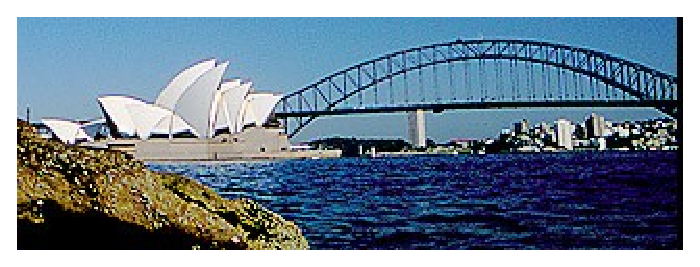
\includegraphics{visitors_guide}

    \vspace{3em}
    \begin{tabular}{lrl}
    {\huge Workshop:}  & {\huge 10 \& 11} & {\huge December 2005}\\[1em]
    {\huge Tutorials:} & {\huge 9} & {\huge December 2005}\\
                       & \multicolumn{1}{l}{Dialog Systems}\\
                       & \multicolumn{1}{l}{Conditional Random Fields}\\
                       & \multicolumn{1}{l}{Tree-Adjoining Grammar}\\
                       & \multicolumn{1}{l}{Document Summarisation}\\[1em]
    {\huge Location:}  & \multicolumn{2}{r}{\huge University of Sydney}\\[1em]
    \end{tabular}
    \vspace{2em}

    {\Large http://www.alta.asn.au/events/altw2005/}
    \vspace{6em}

    \begin{tabular}{c@{\hspace{1cm}}c@{\hspace{1cm}}c}
    \raisebox{-1.3em}{
\includegraphics{logo_sm}} & 
    
\includegraphics[width=6cm]{usyd} & 
    
\includegraphics[width=6cm]{appen} \\[1.8em]
    
\includegraphics[width=2.5cm]{CSIRO_logo_CMYK_colour} &
    
\includegraphics[width=6cm]{DSTO_black_horizontal_logo} &
    
\includegraphics[width=6cm]{NICTA}
    \end{tabular}
  \end{center}}
}}\hfill\mbox{}\\[0.2cm]
%\vspace*{1.3cm}

\end{document}
